% Chapter 3

\chapter{Hybrid Methods} % Main chapter title

\label{Chapter3} % For referencing the chapter elsewhere, use \ref{Chapter2} 
%%%%%%%%%%%%%%%%%%%%%%%%%%%%%%%%%%%%%%%%%%%%%%%%%%%%%%%%%%%%%%%%%%%%%%%%%%%%%%%

%%%%%%%%%%%%%%%%%%%%%%%%%%%%%%%%%%%%%%%%%%%%%%%%%%%%%%%%%%%%%%%%%%%%%%%%%%%%%%%
Quantum computers are not mature enough to solve real-world problems. For instance, the embedding of a QUBO problem into the architecture of a quantum annealer impose a big constraint in the number of variables our problem can have. For this reason, a \textit{hybrid quantum-classical} (HQC) approach is currently the best method one can use to solve large-scale problems, by combining quantum and classical solvers.\\\\
The aim of HQC approaches is to decompose a problem into a \textit{sub-problem(s)} (SP(s)) and \textit{master problem} (MP), so hopefully one of these problems is suitable for a quantum computer, e.g., a quantum annealer would receive a QUBO problem or a problem that can be cast into it, meanwhile the rest of the problems are solved by the classical solver using cutting-edge algorithms. In the present work the problem we are interested in are MILP problems.\\\\
MILP problems can be written as function of decision variables $\textbf{x}$ and complicated decision variables $\textbf{y}$
\begin{equation}
\label{eq: MILP}
    \min_{\textbf{x},\textbf{y}} \textbf{c}^\intercal\textbf{x} + \textbf{d}^\intercal\textbf{y}
\end{equation}
subject to a set of linear constraints,
\begin{align}
    \textbf{A}\textbf{x} + \textbf{B}\textbf{y} \geq \textbf{b}
\end{align}
with $\textbf{c}\in\mathbb{R}^{l_{x}}$, $\textbf{d}\in\mathbb{R}^{l_{y}}$, $\textbf{b}\in\mathbb{R}^{l_{c}}$, $\textbf{x}\in\mathbb{R}_{+}^{l_{x}}$, $\textbf{y}\in\mathbb{R}^{l_{y}}$, $\textbf{A}\in \mathbb{R}^{l_{c}\times l_{x}}$ and $\textbf{B}\in\mathbb{R}^{l_{c}\times l_{y}}$ where $l_{x}$, $l_{y}$ and $l_{c}$ indicate the number of the decision variables $\textbf{x}$, complicated decision variables $\textbf{y}$ -- restricted to the set $\mathbb{Y}$ -- and constraints terms, respectively. 
In many fields, such as the energy sector, quadratic problems are often linearized by casting them into MILP problems. Despite the simplicity of MILP problems they appear in a wide range of real-world applications. They scale badly as the problem size grows, which implies a huge demand of computational resources, which leads to a reduction of the spatial and time resolution. There are classical solvers such as Gurobi\,\cite{gurobi}, CPLEX\,\cite{cplex2009v12} or cbc\,\cite{cbc} that are being used to solve MILP problems and other type of combinatorial problems. However, there are problems for which the best of these solvers -- Gurobi -- exceed the run-time, see Ref.\,\cite{Fernandez-Campoamor2021CommunityAnnealing}. Currently, the scope and granularity of the models
are reduced using clustering algorithms. For this reason, any computational time reduction will have substantial implications in closing the granularity gap between what the current models can solve and the desired resolution needed by energy system operators. It is though that quantum computers could offer advantage over the classical solver in the future though its current state force us to use HQC approaches instead of a pure quantum solver.

%%%%%%%%%%%%%%%%%%%%%%%%%%%%%%%%%%%%%%%%%%%%%%%%%%%%%%%%%%%%%%%%%%%%%%%%%%%%%%%
\section{Classical Benders Decomposition}
The main idea behind \textit{classical Benders decomposition} (CBD) is to decompose the original problem into several sub-problems once the complicated variables are detected. Furthermore, by fixing the complicated variables the problem is simplified. For this reason, CBD decompose the general problem \eqref{eq: MILP} into a MP with integer variables and a SP with the complicated variables fixed by the MP, then both problems are solved interactively until a stopping criterion is satisfied. The convergence of CBD\,\cite{Sahinidis1991BDConvergence} guarantees that we reach the minimum value after a number of iterations. The solution of the master problem generates a lower bound, meanwhile the solution of the sub-problem generate an upper bound. Both problems are solved interactively until lower $L$ and upper $U$ bound satisfy a given threshold $U - L = \epsilon$.\\\\
As an example, consider a general expansion planning problem with cost function given by
\begin{equation}
    \min_{x_{3},g_{1}(h),g_{2}(h),g_{3}(h)}\underbrace{30000x_{3}}_{\text{Investment Cost}} + \underbrace{\sum_{h}10g_{1}(h)+20g_{2}(h) + 5g_{3}(h)}_{\text{Operational Cost}}\\ 
\end{equation}
subject to a set of constraints,
\begin{align}
    0 \leq g_{1}(h) \leq 100, \quad \forall\,h\\
    0 \leq g_{1}(h) \leq 200, \quad \forall\,h\\
    0 \leq g_{2}(h) \leq x_{3}, \quad \forall\,h \\
    D(h) = g_{1}(h) + g_{2}(h) + g_{3}(h), \quad \forall\,h \\
    x_{3} \geq 0
\end{align}
where $x_{3}$ represent the decision of creating a new element $g_{3}$, $h$ represents the snapshot considered and $D(h)$ represents a demand to be fulfilled by the elements $\{g_{j}\}$ at snapshot $h$. Notice, that if we just look to the investment cost, then we $x_{3}$ would be set to zero. However, the operational cost of the element $g_{3}$ is cheaper than the other elements. Moreover, notice that if we consider a large set of snapshots $h$, then the operational cost is the dominant term. Analogously, for a short set of snapshots the investment cost is the dominant term of the cost function. In summary, extremal solutions lead to a high value of cost function in one of this ways
\begin{itemize}
    \item \textbf{Underinvestment} leads to a high value of the total cost function because the system is not able to fulfill the demand $D(h)$.
    \item \textbf{Overinvestment} leads to a high value of the total cost function despite it fulfill the demand. Intuitively, we are creating more elements $\{g_{j}\}$ than we need. Usually there is an upper bound due to capital budget.
\end{itemize}
The optimization problem is a trade-off between operational cost and investment cost where the optimal solution minimize the investment cost and operational cost fulfilling at the same time the constraints of the problem.
%%%%%%%%%%%%%%%%%%%%%%%%%%%%%%%%%%%%%%%%%%%%%%
\subsection{Complicated variables}
We can consider a decision variable to be complicated if the decision variable is involved in most of the constraints or the decision variable produce non-convex optimization problems. For instance, suppose that the decision variable $x_{3}$ of the previous cost function is a complicated variable. Fixing that variable and considering a single snapshot $h=1$ would allow us to re-write the problem 
\begin{equation}
    \min_{g_{1}(1), g_{2}(1), g_{3}(1)} \sum_{h}10g_{1}(1)+20g_{2}(1) + 5g_{3}(1)
\end{equation}
subject to
\begin{align}
    0 \leq g_{1}(1) \leq 100 \\
    0 \leq g_{1}(1) \leq 200 \\
    0 \leq g_{2}(1) \leq x_{3}^{(\text{fixed})} \\
    D(h) = g_{1}(1) + g_{2}(1) + g_{3}(1)
\end{align}
\begin{figure}[H]
\centering
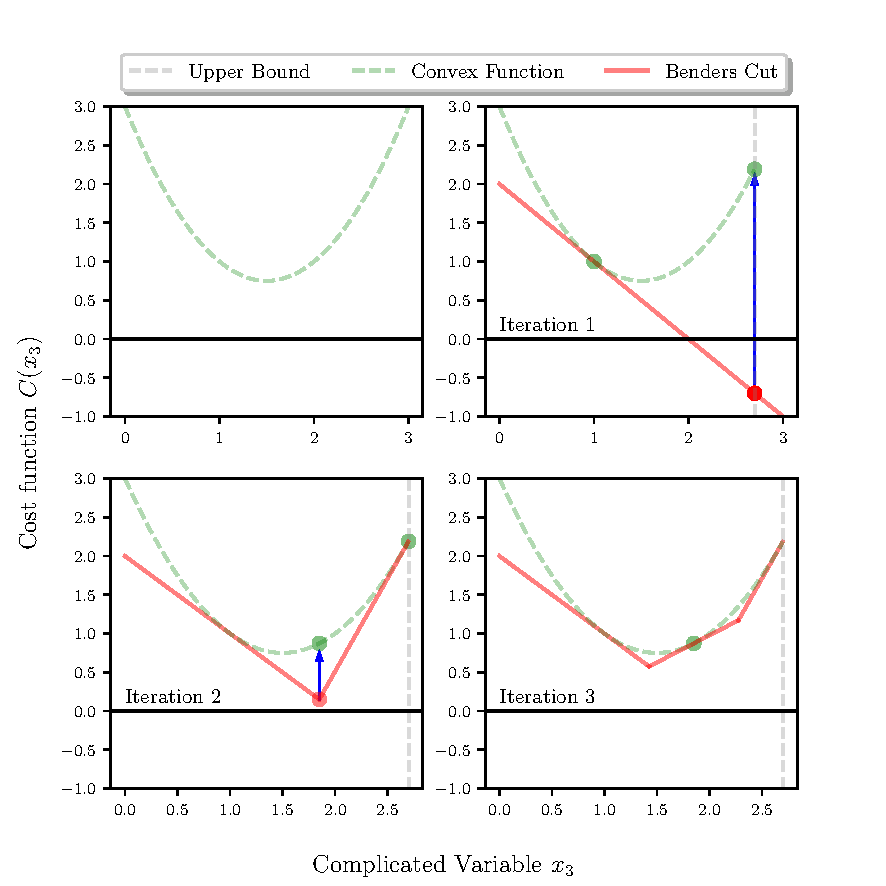
\includegraphics[width=\textwidth]{Figures/BenderIlustration.pdf} 
\caption{Benders cuts.}
\label{fig:BDIlustration}
\end{figure}

\subsection{Upper and Lower Bounds}
%%%%%%%%%%%%%%%%%%%%%%%%%%%%%%%%%%%%%%%%%%%%%%%%%%%%%%%%%%%%%%%%%%%%%%%%%%%%%%%
% QA + SA
%%%%%%%%%%%%%%%%%%%%%%%%%%%%%%%%%%%%%%%%%%%%%%%%%%%%%%%%%%%%%%%%%%%%%%%%%%%%%%%
\section{Hybrid classical-quantum annealing algorithm}
In Appx.\,\ref{AppendixB}, we show the foundations of \textit{simulated annealing} algorithm (SA) and solve a travelling salesman problem to illustrate it. A simulated annealing algorithm does not guarantee to get the optimal solution but the results we can get with a good annealing schedule are good enough in accuracy and time. Analogously with a quantum annealing algorithm. In this section, we illustrate the decomposition of a QUBO problem into two parts. A sub-problem solved by simulated annealing on a classical solver. A master problem addressed to a quantum annealer such that a embedding is possible.
%%%%%%%%%%%%%%%%%%%%%%%%%%%%%%%%%%%%%%%%%%%%%%%%%%%%%%%%%%%%%%%%%%%%%%%%%%%%%%%
\subsection{SA-QA protocol}
The hybrid quantum-classical algorithm based on combining SA with QA is inspired on\,\cite{Ding2019ImplementationDesign}. In that work, the authors proposed the following structure of the hybrid algorithm for a QUBO problem:
\begin{figure}[H]
\centering
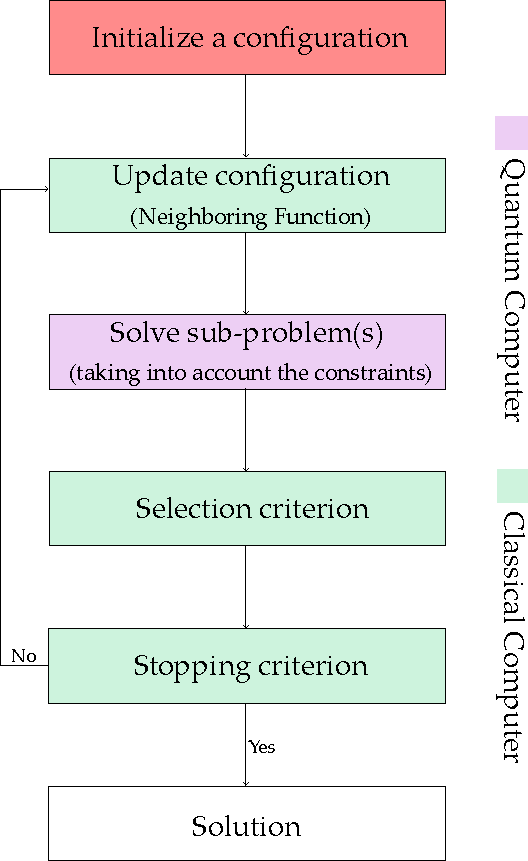
\includegraphics[width=0.5\textwidth]{Figures/SAQAProtocol_Layer 1.pdf} 
\caption{SA-QA protocol scheme.}
\label{fig:SA_QAProtocol}
\end{figure}
\begin{enumerate}
    \item Set the cost to a high value and initialize a configuration for the problem, i.e., annealing schedule, initial and final temperature, and a selection criterion.
    \item Randomly generate a new configuration by changing the values of the binary variables according to a neighboring function that generate a new configuration in one of this ways:
    \begin{enumerate}
        \item Randomly pick a binary variable with value 1 and set it to 0.
        \item Randomly pick a binary variable with value 0 and set it to 1.
        \item Randomly pick two binary variables with different values and swap them.
    \end{enumerate}
    \item Given the new configuration, solve the operational cost problem taking into account the constraints with a quantum annealing algorithm.
    \item Apply the selection criterion to keep or to discard the current configuration.
    \item Repeat steps 2 to 4 until a iteration index is equal to the upper value, then decrease the temperature and reset the iteration index.
    \item Outputs the current cost function value and its solution $\vec{x}$ when a stopping criterion is satisfied.
\end{enumerate}
Notice that the algorithm solve the master problem with a simulating annealing algorithm in a classical solver and then the sub-problem(s) -- which carries the constraints -- with the quantum computer, more precisely with a quantum annealer. For this reason, the sub-problem(s) must have binary constraints or integer if we do not want to deal with discretization errors. Hence, the approach as stated before is not for problems whose sub-problem(s) has real constraints meanwhile the master problem is more suitable for a quantum annealer.\\\\
In order to apply both simulated and quantum annealing to problems with real constraints, we have to reconsider or adapt the previous scheme.
%%%%%%%%%%%%%%%%%%%%%%%%%%%%%%%%%%%%%%%%%%%%%%%%%%%%%%%%%%%%%%%%%%%%%%%%%%%%%%%
% BD: Multi-Cuts
%%%%%%%%%%%%%%%%%%%%%%%%%%%%%%%%%%%%%%%%%%%%%%%%%%%%%%%%%%%%%%%%%%%%%%%%%%%%%%%
\subsection{Hybrid Quantum-Classical Multi-cut Benders Approach}
In this section we present the protocol of a hybrid quantum-classical approach that has been applied to power system applications, see Ref.\,\cite{Paterakis2021HybridApplication}.\\\\


%----------------------------------------------------------------------------------------

% Define some commands to keep the formatting separated from the content 
\newcommand{\keyword}[1]{\textbf{#1}}
\newcommand{\tabhead}[1]{\textbf{#1}}
\newcommand{\code}[1]{\texttt{#1}}
\newcommand{\file}[1]{\texttt{\bfseries#1}}
\newcommand{\option}[1]{\texttt{\itshape#1}}

%----------------------------------------------------------------------------------------



